\section[Cohomology of unitarizable modules for An, 1 < n < 6]{Cohomology of unitarizable modules for $A_n$, $2 \leq n \leq 5$}

\subsection[su(1,1): 1,1,1]{$\boldsymbol{\mathfrak{su}(1, 1)\!:\; p'= 1,\, q' = 1,\, l = 1}$}

Cone of unitarizable weights: $0$ \\


\begin{figure}[H]
  \centering
      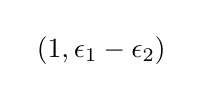
\begin{tikzpicture}[>=latex,line join=bevel,]
%%
\node (node_0) at (27.0bp,8.5bp) [draw,draw=none] {$(1, \epsilon_{1} - \epsilon_{2})$};
%
\end{tikzpicture}
  \caption{Nonnegative scalar products with noncompact roots}
\end{figure}

%\noindent $\lambda = $ $0$ \\
\noindent Set of singular roots: $\emptyset$ \\

\begin{figure}[H]
  \centering
  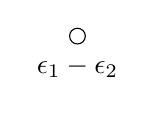
\begin{tikzpicture}
\draw[fill=white] (0 cm, 0 cm) circle (.1cm) node[below=4pt]{$\epsilon_{1} - \epsilon_{2}$};
\end{tikzpicture}
  \caption{The reduced hermitian symmetric pair $(\mathfrak{g}_\lambda, \mathfrak{k}_\lambda)$}
\end{figure}

\begin{figure}[H]
  \centering
      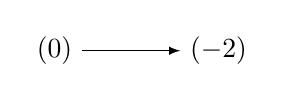
\begin{tikzpicture}[>=latex,line join=bevel,]
%%
\node (node_1) at (9.5bp,8.5bp) [draw,draw=none] {$\left(0\right)$};
  \node (node_0) at (68.5bp,8.5bp) [draw,draw=none] {$\left(-2\right)$};
  \draw [black,->] (node_1) ..controls (26.173bp,8.5bp) and (35.797bp,8.5bp)  .. (node_0);
%
\end{tikzpicture}
  \caption{Nilpotent cohomology / BGG resolution}
\end{figure}

        


\subsection[su(1,2): 1,1,1]{$\boldsymbol{\mathfrak{su}(1, 2)\!:\; p'= 1,\, q' = 1,\, l = 1}$}

Cone of unitarizable weights: $-\left(a_{2} + 2\right)\omega_{1} + \left(a_{2} + 1\right)\omega_{2}$ \\


\begin{figure}[H]
  \centering
      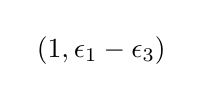
\begin{tikzpicture}[>=latex,line join=bevel,]
%%
\node (node_0) at (27.0bp,8.5bp) [draw,draw=none] {$(1, \epsilon_{1} - \epsilon_{3})$};
%
\end{tikzpicture}
  \caption{Nonnegative scalar products with noncompact roots}
\end{figure}
    

%\noindent $\lambda = $ $-\left(a_{2} + 2\right)\omega_{1} + \left(a_{2} + 1\right)\omega_{2}$ \\
\noindent Set of singular roots: $\emptyset$ \\

\begin{figure}[H]
  \centering
  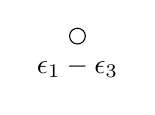
\begin{tikzpicture}
\draw[fill=white] (0 cm, 0 cm) circle (.1cm) node[below=4pt]{$\epsilon_{1} - \epsilon_{3}$};
\end{tikzpicture}
  \caption{The reduced hermitian symmetric pair $(\mathfrak{g}_\lambda, \mathfrak{k}_\lambda)$}
\end{figure}

\begin{figure}[H]
  \centering
      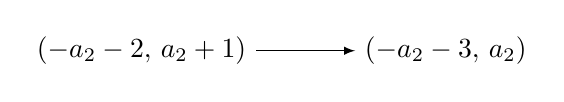
\begin{tikzpicture}[>=latex,line join=bevel,]
%%
\node (node_1) at (41.0bp,8.5bp) [draw,draw=none] {$\left(-a_{2} - 2,\,a_{2} + 1\right)$};
  \node (node_0) at (150.5bp,8.5bp) [draw,draw=none] {$\left(-a_{2} - 3,\,a_{2}\right)$};
  \draw [black,->] (node_1) ..controls (90.432bp,8.5bp) and (99.314bp,8.5bp)  .. (node_0);
%
\end{tikzpicture}
  \caption{Nilpotent cohomology / BGG resolution}
\end{figure}

        


\subsection[su(1,2): 1,2,1]{$\boldsymbol{\mathfrak{su}(1, 2)\!:\; p'= 1,\, q' = 2,\, l = 1}$}

Cone of unitarizable weights: $0$ \\

\begin{figure}[H]
  \centering
      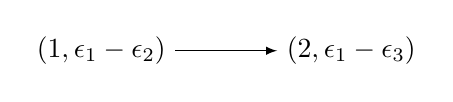
\begin{tikzpicture}[>=latex,line join=bevel,]
%%
\node (node_1) at (117.0bp,8.5bp) [draw,draw=none] {$(2, \epsilon_{1} - \epsilon_{3})$};
  \node (node_0) at (27.0bp,8.5bp) [draw,draw=none] {$(1, \epsilon_{1} - \epsilon_{2})$};
  \draw [black,->] (node_0) ..controls (62.393bp,8.5bp) and (71.311bp,8.5bp)  .. (node_1);
%
\end{tikzpicture}
  \caption{Nonnegative scalar products with noncompact roots}
\end{figure}

%\noindent $\lambda = $ $0$ \\
\noindent Set of singular roots: $\emptyset$ \\

\begin{figure}[H]
  \centering
  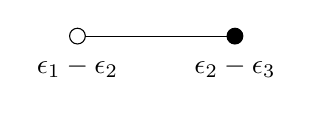
\begin{tikzpicture}
\draw (0 cm,0) -- (2 cm,0);
\draw[fill=white] (0 cm, 0 cm) circle (.1cm) node[below=4pt]{$\epsilon_{1} - \epsilon_{2}$};
\draw[fill=black] (2 cm, 0 cm) circle (.1cm) node[below=4pt]{$\epsilon_{2} - \epsilon_{3}$};
\end{tikzpicture}
  \caption{The reduced hermitian symmetric pair $(\mathfrak{g}_\lambda, \mathfrak{k}_\lambda)$}
\end{figure}

\begin{figure}[H]
  \centering
      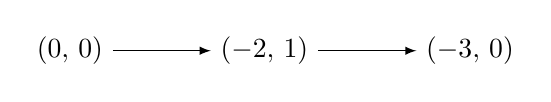
\begin{tikzpicture}[>=latex,line join=bevel,]
%%
\node (node_2) at (15.0bp,8.5bp) [draw,draw=none] {$\left(0,\,0\right)$};
  \node (node_1) at (159.0bp,8.5bp) [draw,draw=none] {$\left(-3,\,0\right)$};
  \node (node_0) at (85.0bp,8.5bp) [draw,draw=none] {$\left(-2,\,1\right)$};
  \draw [black,->] (node_0) ..controls (111.87bp,8.5bp) and (121.03bp,8.5bp)  .. (node_1);
  \draw [black,->] (node_2) ..controls (37.527bp,8.5bp) and (46.927bp,8.5bp)  .. (node_0);
%
\end{tikzpicture}
  \caption{Nilpotent cohomology / BGG resolution}
\end{figure}

        


\subsection[su(1,3): 1,1,1]{$\boldsymbol{\mathfrak{su}(1, 3)\!:\; p'= 1,\, q' = 1,\, l = 1}$}

Cone of unitarizable weights: $-\left(a_{2} + a_{3} + 3\right)\omega_{1} + \left(a_{3} + 1\right)\omega_{3}$ \\


\begin{figure}[H]
  \centering
      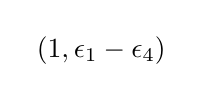
\begin{tikzpicture}[>=latex,line join=bevel,]
%%
\node (node_0) at (27.0bp,8.5bp) [draw,draw=none] {$(1, \epsilon_{1} - \epsilon_{4})$};
%
\end{tikzpicture}
  \caption{Nonnegative scalar products with noncompact roots}
\end{figure}
    

%\noindent $\lambda = $ $-\left(a_{2} + a_{3} + 3\right)\omega_{1} + \left(a_{3} + 1\right)\omega_{3}$ \\
\noindent Set of singular roots: $\emptyset$ \\

\begin{figure}[H]
  \centering
  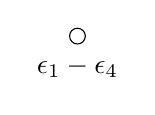
\begin{tikzpicture}
\draw[fill=white] (0 cm, 0 cm) circle (.1cm) node[below=4pt]{$\epsilon_{1} - \epsilon_{4}$};
\end{tikzpicture}
  \caption{The reduced hermitian symmetric pair $(\mathfrak{g}_\lambda, \mathfrak{k}_\lambda)$}
\end{figure}

\begin{figure}[H]
  \centering
      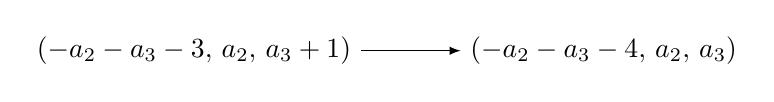
\begin{tikzpicture}[>=latex,line join=bevel,]
%%
\node (node_1) at (207.5bp,8.5bp) [draw,draw=none] {$\left(-a_{2} - a_{3} - 4,\,a_{2},\,a_{3}\right)$};
  \node (node_0) at (60.0bp,8.5bp) [draw,draw=none] {$\left(-a_{2} - a_{3} - 3,\,a_{2},\,a_{3} + 1\right)$};
  \draw [black,->] (node_0) ..controls (128.57bp,8.5bp) and (137.21bp,8.5bp)  .. (node_1);
%
\end{tikzpicture}
  \caption{Nilpotent cohomology / BGG resolution}
\end{figure}

        


\subsection[su(1,3): 1,2,1]{$\boldsymbol{\mathfrak{su}(1, 3)\!:\; p'= 1,\, q' = 2,\, l = 1}$}

Cone of unitarizable weights: $-\left(a_{2} + 2\right)\omega_{1} + \left(a_{2} + 1\right)\omega_{2}$ \\


\begin{figure}[H]
  \centering
      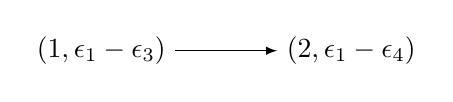
\begin{tikzpicture}[>=latex,line join=bevel,]
%%
\node (node_1) at (117.0bp,8.5bp) [draw,draw=none] {$(2, \epsilon_{1} - \epsilon_{4})$};
  \node (node_0) at (27.0bp,8.5bp) [draw,draw=none] {$(1, \epsilon_{1} - \epsilon_{3})$};
  \draw [black,->] (node_0) ..controls (62.393bp,8.5bp) and (71.311bp,8.5bp)  .. (node_1);
%
\end{tikzpicture}
  \caption{Nonnegative scalar products with noncompact roots}
\end{figure}
    

%\noindent $\lambda = $ $-\left(a_{2} + 2\right)\omega_{1} + \left(a_{2} + 1\right)\omega_{2}$ \\
\noindent Set of singular roots: $\emptyset$ \\

\begin{figure}[H]
  \centering
  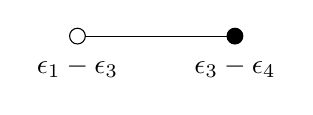
\begin{tikzpicture}
\draw (0 cm,0) -- (2 cm,0);
\draw[fill=white] (0 cm, 0 cm) circle (.1cm) node[below=4pt]{$\epsilon_{1} - \epsilon_{3}$};
\draw[fill=black] (2 cm, 0 cm) circle (.1cm) node[below=4pt]{$\epsilon_{3} - \epsilon_{4}$};
\end{tikzpicture}
  \caption{The reduced hermitian symmetric pair $(\mathfrak{g}_\lambda, \mathfrak{k}_\lambda)$}
\end{figure}

\begin{figure}[H]
  \centering
      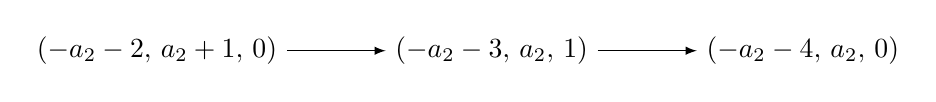
\begin{tikzpicture}[>=latex,line join=bevel,]
%%
\node (node_2) at (279.0bp,8.5bp) [draw,draw=none] {$\left(-a_{2} - 4,\,a_{2},\,0\right)$};
  \node (node_1) at (167.0bp,8.5bp) [draw,draw=none] {$\left(-a_{2} - 3,\,a_{2},\,1\right)$};
  \node (node_0) at (46.5bp,8.5bp) [draw,draw=none] {$\left(-a_{2} - 2,\,a_{2} + 1,\,0\right)$};
  \draw [black,->] (node_0) ..controls (101.65bp,8.5bp) and (110.36bp,8.5bp)  .. (node_1);
  \draw [black,->] (node_1) ..controls (213.39bp,8.5bp) and (222.13bp,8.5bp)  .. (node_2);
%
\end{tikzpicture}
  \caption{Nilpotent cohomology / BGG resolution}
\end{figure}

        


\subsection[su(1,3): 1,3,1]{$\boldsymbol{\mathfrak{su}(1, 3)\!:\; p'= 1,\, q' = 3,\, l = 1}$}

Cone of unitarizable weights: $0$ \\

\begin{figure}[H]
  \centering
      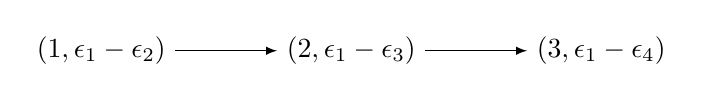
\begin{tikzpicture}[>=latex,line join=bevel,]
%%
\node (node_2) at (207.0bp,8.5bp) [draw,draw=none] {$(3, \epsilon_{1} - \epsilon_{4})$};
  \node (node_1) at (117.0bp,8.5bp) [draw,draw=none] {$(2, \epsilon_{1} - \epsilon_{3})$};
  \node (node_0) at (27.0bp,8.5bp) [draw,draw=none] {$(1, \epsilon_{1} - \epsilon_{2})$};
  \draw [black,->] (node_0) ..controls (62.393bp,8.5bp) and (71.311bp,8.5bp)  .. (node_1);
  \draw [black,->] (node_1) ..controls (152.39bp,8.5bp) and (161.31bp,8.5bp)  .. (node_2);
%
\end{tikzpicture}
  \caption{Nonnegative scalar products with noncompact roots}
\end{figure}

%\noindent $\lambda = $ $0$ \\
\noindent Set of singular roots: $\emptyset$ \\

\begin{figure}[H]
  \centering
  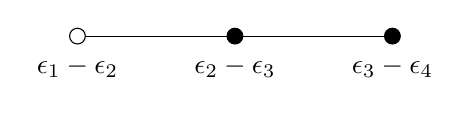
\begin{tikzpicture}
\draw (0 cm,0) -- (4 cm,0);
\draw[fill=white] (0 cm, 0 cm) circle (.1cm) node[below=4pt]{$\epsilon_{1} - \epsilon_{2}$};
\draw[fill=black] (2 cm, 0 cm) circle (.1cm) node[below=4pt]{$\epsilon_{2} - \epsilon_{3}$};
\draw[fill=black] (4 cm, 0 cm) circle (.1cm) node[below=4pt]{$\epsilon_{3} - \epsilon_{4}$};
\end{tikzpicture}
  \caption{The reduced hermitian symmetric pair $(\mathfrak{g}_\lambda, \mathfrak{k}_\lambda)$}
\end{figure}

\begin{figure}[H]
  \centering
      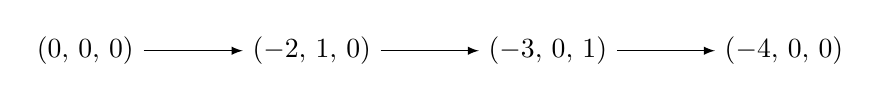
\begin{tikzpicture}[>=latex,line join=bevel,]
%%
\node (node_3) at (102.5bp,8.5bp) [draw,draw=none] {$\left(-2,\,1,\,0\right)$};
  \node (node_2) at (272.5bp,8.5bp) [draw,draw=none] {$\left(-4,\,0,\,0\right)$};
  \node (node_1) at (21.0bp,8.5bp) [draw,draw=none] {$\left(0,\,0,\,0\right)$};
  \node (node_0) at (187.5bp,8.5bp) [draw,draw=none] {$\left(-3,\,0,\,1\right)$};
  \draw [black,->] (node_1) ..controls (49.779bp,8.5bp) and (58.821bp,8.5bp)  .. (node_3);
  \draw [black,->] (node_3) ..controls (135.04bp,8.5bp) and (144.1bp,8.5bp)  .. (node_0);
  \draw [black,->] (node_0) ..controls (220.04bp,8.5bp) and (229.1bp,8.5bp)  .. (node_2);
%
\end{tikzpicture}
  \caption{Nilpotent cohomology / BGG resolution}
\end{figure}

        


\subsection[su(2,2): 1,1,1]{$\boldsymbol{\mathfrak{su}(2, 2)\!:\; p'= 1,\, q' = 1,\, l = 1}$}

Cone of unitarizable weights: $\left(a_{1} + 1\right)\omega_{1} - \left(a_{1} + a_{3} + 4\right)\omega_{2} + \left(a_{3} + 1\right)\omega_{3}$ \\


\begin{figure}[H]
  \centering
      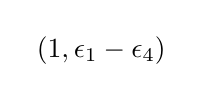
\begin{tikzpicture}[>=latex,line join=bevel,]
%%
\node (node_0) at (27.0bp,8.5bp) [draw,draw=none] {$(1, \epsilon_{1} - \epsilon_{4})$};
%
\end{tikzpicture}
  \caption{Nonnegative scalar products with noncompact roots}
\end{figure}
    

%\noindent $\lambda = $ $\left(a_{1} + 1\right)\omega_{1} - \left(a_{1} + a_{3} + 4\right)\omega_{2} + \left(a_{3} + 1\right)\omega_{3}$ \\
\noindent Set of singular roots: $\emptyset$ \\

\begin{figure}[H]
  \centering
  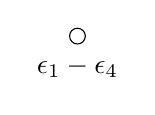
\begin{tikzpicture}
\draw[fill=white] (0 cm, 0 cm) circle (.1cm) node[below=4pt]{$\epsilon_{1} - \epsilon_{4}$};
\end{tikzpicture}
  \caption{The reduced hermitian symmetric pair $(\mathfrak{g}_\lambda, \mathfrak{k}_\lambda)$}
\end{figure}

\begin{figure}[H]
  \centering
      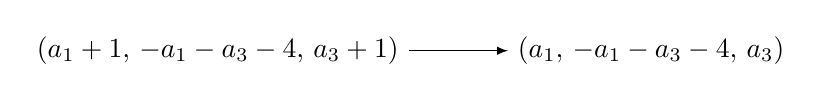
\begin{tikzpicture}[>=latex,line join=bevel,]
%%
\node (node_1) at (224.5bp,8.5bp) [draw,draw=none] {$\left(a_{1},\,-a_{1} - a_{3} - 4,\,a_{3}\right)$};
  \node (node_0) at (68.5bp,8.5bp) [draw,draw=none] {$\left(a_{1} + 1,\,-a_{1} - a_{3} - 4,\,a_{3} + 1\right)$};
  \draw [black,->] (node_0) ..controls (145.55bp,8.5bp) and (154.21bp,8.5bp)  .. (node_1);
%
\end{tikzpicture}
  \caption{Nilpotent cohomology / BGG resolution}
\end{figure}

        


\subsection[su(2,2): 1,2,1]{$\boldsymbol{\mathfrak{su}(2, 2)\!:\; p'= 1,\, q' = 2,\, l = 1}$}

Cone of unitarizable weights: $\left(a_{1} + 1\right)\omega_{1} - \left(a_{1} + 2\right)\omega_{2}$ \\


\begin{figure}[H]
  \centering
      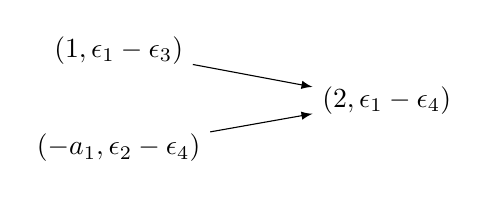
\begin{tikzpicture}[>=latex,line join=bevel,]
%%
\node (node_2) at (130.0bp,25.5bp) [draw,draw=none] {$(2, \epsilon_{1} - \epsilon_{4})$};
  \node (node_1) at (33.5bp,8.5bp) [draw,draw=none] {$(-a_{1}, \epsilon_{2} - \epsilon_{4})$};
  \node (node_0) at (33.5bp,43.5bp) [draw,draw=none] {$(1, \epsilon_{1} - \epsilon_{3})$};
  \draw [black,->] (node_0) ..controls (70.509bp,36.641bp) and (82.02bp,34.449bp)  .. (node_2);
  \draw [black,->] (node_1) ..controls (75.372bp,15.853bp) and (84.404bp,17.478bp)  .. (node_2);
%
\end{tikzpicture}
  \caption{Nonnegative scalar products with noncompact roots}
\end{figure}
    

\noindent $\lambda = \omega_{1} - 2\omega_{2}$ \\
\noindent Set of singular roots: $\{\epsilon_{2} - \epsilon_{4}$\} \\

\begin{figure}[H]
  \centering
  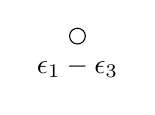
\begin{tikzpicture}
\draw[fill=white] (0 cm, 0 cm) circle (.1cm) node[below=4pt]{$\epsilon_{1} - \epsilon_{3}$};
\end{tikzpicture}
  \caption{The reduced hermitian symmetric pair $(\mathfrak{g}_\lambda, \mathfrak{k}_\lambda)$}
\end{figure}

\begin{figure}[H]
  \centering
      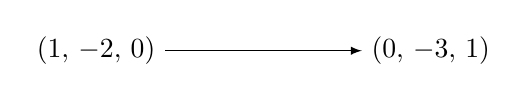
\begin{tikzpicture}[>=latex,line join=bevel,]
%%
\node (node_1) at (46.5bp,8.5bp) [draw,draw=none] {$\left( 1,\,- 2,\,0\right)$};
  \node (node_0) at (167.0bp,8.5bp) [draw,draw=none] {$\left(0,\, - 3,\,1\right)$};
  \draw [black,->] (node_1) ..controls (101.65bp,8.5bp) and (110.36bp,8.5bp)  .. (node_0);
%
\end{tikzpicture}
  \caption{Nilpotent cohomology / BGG resolution}
\end{figure}

\noindent $\lambda = \left(a_{1} + 1\right)\omega_{1} - \left(a_{1} + 2\right)\omega_{2}$, $a_1 \geq 1$ \\
\noindent Set of singular roots: $\emptyset$ \\

\begin{figure}[H]
  \centering
  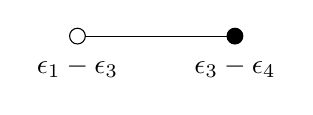
\begin{tikzpicture}
\draw (0 cm,0) -- (2 cm,0);
\draw[fill=white] (0 cm, 0 cm) circle (.1cm) node[below=4pt]{$\epsilon_{1} - \epsilon_{3}$};
\draw[fill=black] (2 cm, 0 cm) circle (.1cm) node[below=4pt]{$\epsilon_{3} - \epsilon_{4}$};
\end{tikzpicture}
  \caption{The reduced hermitian symmetric pair $(\mathfrak{g}_\lambda, \mathfrak{k}_\lambda)$}
\end{figure}

\begin{figure}[H]
  \centering
      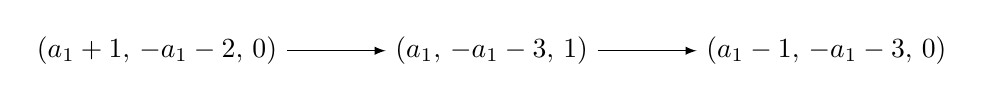
\begin{tikzpicture}[>=latex,line join=bevel,]
%%
\node (node_2) at (287.5bp,8.5bp) [draw,draw=none] {$\left(a_{1} - 1,\,-a_{1} - 3,\,0\right)$};
  \node (node_1) at (167.0bp,8.5bp) [draw,draw=none] {$\left(a_{1},\,-a_{1} - 3,\,1\right)$};
  \node (node_0) at (46.5bp,8.5bp) [draw,draw=none] {$\left(a_{1} + 1,\,-a_{1} - 2,\,0\right)$};
  \draw [black,->] (node_0) ..controls (101.65bp,8.5bp) and (110.36bp,8.5bp)  .. (node_1);
  \draw [black,->] (node_1) ..controls (213.27bp,8.5bp) and (222.01bp,8.5bp)  .. (node_2);
%
\end{tikzpicture}
  \caption{Nilpotent cohomology / BGG resolution}
\end{figure}        


\subsection[su(2,2): 2,1,1]{$\boldsymbol{\mathfrak{su}(2, 2)\!:\; p'= 2,\, q' = 1,\, l = 1}$}

Cone of unitarizable weights: $-\left(a_{3} + 2\right)\omega_{2} + \left(a_{3} + 1\right)\omega_{3}$ \\


\begin{figure}[H]
  \centering
      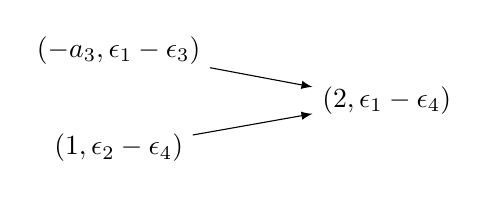
\begin{tikzpicture}[>=latex,line join=bevel,]
%%
\node (node_2) at (33.5bp,8.5bp) [draw,draw=none] {$(1, \epsilon_{2} - \epsilon_{4})$};
  \node (node_1) at (33.5bp,43.5bp) [draw,draw=none] {$(-a_{3}, \epsilon_{1} - \epsilon_{3})$};
  \node (node_0) at (130.0bp,25.5bp) [draw,draw=none] {$(2, \epsilon_{1} - \epsilon_{4})$};
  \draw [black,->] (node_2) ..controls (70.509bp,14.978bp) and (82.02bp,17.049bp)  .. (node_0);
  \draw [black,->] (node_1) ..controls (75.372bp,35.715bp) and (84.404bp,33.994bp)  .. (node_0);
%
\end{tikzpicture}
  \caption{Nonnegative scalar products with noncompact roots}
\end{figure}
    

\noindent $\lambda = -2\omega_{2} + \omega_{3}$ \\
\noindent Set of singular roots: $\{\epsilon_{1} - \epsilon_{3}$\} \\

\begin{figure}[H]
  \centering
  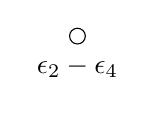
\begin{tikzpicture}
\draw[fill=white] (0 cm, 0 cm) circle (.1cm) node[below=4pt]{$\epsilon_{2} - \epsilon_{4}$};
\end{tikzpicture}
  \caption{The reduced hermitian symmetric pair $(\mathfrak{g}_\lambda, \mathfrak{k}_\lambda)$}
\end{figure}

\begin{figure}[H]
  \centering
      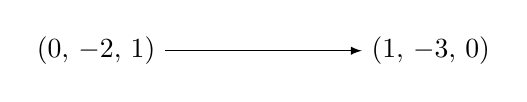
\begin{tikzpicture}[>=latex,line join=bevel,]
%%
\node (node_1) at (167.0bp,8.5bp) [draw,draw=none] {$\left(1,\, - 3,\,0\right)$};
  \node (node_0) at (46.5bp,8.5bp) [draw,draw=none] {$\left(0,\, - 2,\, 1\right)$};
  \draw [black,->] (node_0) ..controls (101.65bp,8.5bp) and (110.36bp,8.5bp)  .. (node_1);
%
\end{tikzpicture}
  \caption{Nilpotent cohomology / BGG resolution}
\end{figure}

\noindent $\lambda = -\left(a_{3} + 2\right)\omega_{2} + \left(a_{3} + 1\right)\omega_{3}$, $a_3 \geq 1$ \\
\noindent Set of singular roots: $\emptyset$ \\

\begin{figure}[H]
  \centering
  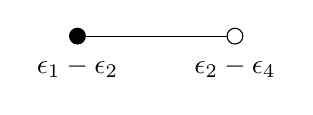
\begin{tikzpicture}
\draw (0 cm,0) -- (2 cm,0);
\draw[fill=black] (0 cm, 0 cm) circle (.1cm) node[below=4pt]{$\epsilon_{1} - \epsilon_{2}$};
\draw[fill=white] (2 cm, 0 cm) circle (.1cm) node[below=4pt]{$\epsilon_{2} - \epsilon_{4}$};
\end{tikzpicture}
  \caption{The reduced hermitian symmetric pair $(\mathfrak{g}_\lambda, \mathfrak{k}_\lambda)$}
\end{figure}

\begin{figure}[H]
  \centering
      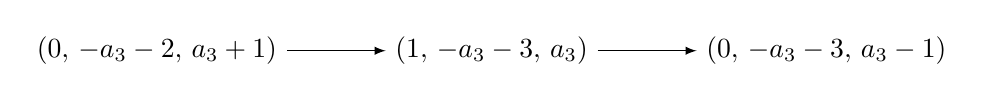
\begin{tikzpicture}[>=latex,line join=bevel,]
%%
\node (node_2) at (46.5bp,8.5bp) [draw,draw=none] {$\left(0,\,-a_{3} - 2,\,a_{3} + 1\right)$};
  \node (node_1) at (287.5bp,8.5bp) [draw,draw=none] {$\left(0,\,-a_{3} - 3,\,a_{3} - 1\right)$};
  \node (node_0) at (167.0bp,8.5bp) [draw,draw=none] {$\left(1,\,-a_{3} - 3,\,a_{3}\right)$};
  \draw [black,->] (node_0) ..controls (213.27bp,8.5bp) and (222.01bp,8.5bp)  .. (node_1);
  \draw [black,->] (node_2) ..controls (101.65bp,8.5bp) and (110.36bp,8.5bp)  .. (node_0);
%
\end{tikzpicture}
  \caption{Nilpotent cohomology / BGG resolution}
\end{figure}        


\subsection[su(2,2): 2,2,1]{$\boldsymbol{\mathfrak{su}(2, 2)\!:\; p'= 2,\, q' = 2,\, l = 1}$}

Cone of unitarizable weights: $0$ \\

\begin{figure}[H]
  \centering
      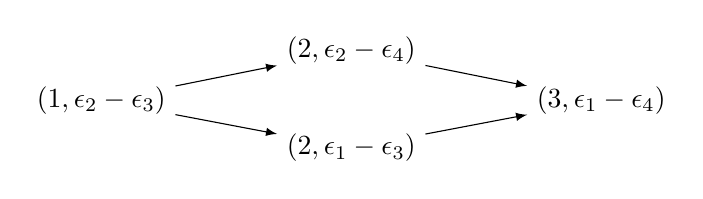
\begin{tikzpicture}[>=latex,line join=bevel,]
%%
\node (node_3) at (117.0bp,43.5bp) [draw,draw=none] {$(2, \epsilon_{2} - \epsilon_{4})$};
  \node (node_2) at (117.0bp,8.5bp) [draw,draw=none] {$(2, \epsilon_{1} - \epsilon_{3})$};
  \node (node_1) at (207.0bp,25.5bp) [draw,draw=none] {$(3, \epsilon_{1} - \epsilon_{4})$};
  \node (node_0) at (27.0bp,25.5bp) [draw,draw=none] {$(1, \epsilon_{2} - \epsilon_{3})$};
  \draw [black,->] (node_0) ..controls (62.481bp,32.553bp) and (71.507bp,34.399bp)  .. (node_3);
  \draw [black,->] (node_2) ..controls (152.39bp,15.144bp) and (161.31bp,16.867bp)  .. (node_1);
  \draw [black,->] (node_0) ..controls (62.393bp,18.856bp) and (71.311bp,17.133bp)  .. (node_2);
  \draw [black,->] (node_3) ..controls (152.48bp,36.447bp) and (161.51bp,34.601bp)  .. (node_1);
%
\end{tikzpicture}
  \caption{Nonnegative scalar products with noncompact roots}
\end{figure}

%\noindent $\lambda = $ $0$ \\
\noindent Set of singular roots: $\emptyset$ \\

\begin{figure}[H]
  \centering
  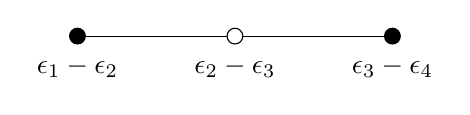
\begin{tikzpicture}
\draw (0 cm,0) -- (4 cm,0);
\draw[fill=black] (0 cm, 0 cm) circle (.1cm) node[below=4pt]{$\epsilon_{1} - \epsilon_{2}$};
\draw[fill=white] (2 cm, 0 cm) circle (.1cm) node[below=4pt]{$\epsilon_{2} - \epsilon_{3}$};
\draw[fill=black] (4 cm, 0 cm) circle (.1cm) node[below=4pt]{$\epsilon_{3} - \epsilon_{4}$};
\end{tikzpicture}
  \caption{The reduced hermitian symmetric pair $(\mathfrak{g}_\lambda, \mathfrak{k}_\lambda)$}
\end{figure}

\begin{figure}[H]
  \centering
      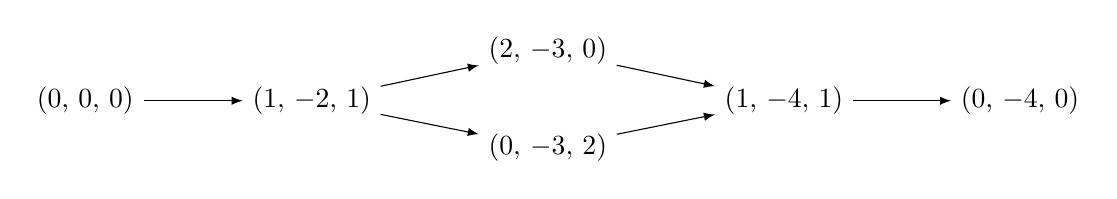
\begin{tikzpicture}[>=latex,line join=bevel,]
%%
\node (node_5) at (272.5bp,25.5bp) [draw,draw=none] {$\left(1,\,-4,\,1\right)$};
  \node (node_4) at (357.5bp,25.5bp) [draw,draw=none] {$\left(0,\,-4,\,0\right)$};
  \node (node_3) at (187.5bp,8.5bp) [draw,draw=none] {$\left(0,\,-3,\,2\right)$};
  \node (node_2) at (21.0bp,25.5bp) [draw,draw=none] {$\left(0,\,0,\,0\right)$};
  \node (node_1) at (102.5bp,25.5bp) [draw,draw=none] {$\left(1,\,-2,\,1\right)$};
  \node (node_0) at (187.5bp,43.5bp) [draw,draw=none] {$\left(2,\,-3,\,0\right)$};
  \draw [black,->] (node_5) ..controls (305.04bp,25.5bp) and (314.1bp,25.5bp)  .. (node_4);
  \draw [black,->] (node_2) ..controls (49.779bp,25.5bp) and (58.821bp,25.5bp)  .. (node_1);
  \draw [black,->] (node_0) ..controls (220.12bp,36.642bp) and (229.3bp,34.651bp)  .. (node_5);
  \draw [black,->] (node_1) ..controls (135.12bp,19.023bp) and (144.3bp,17.143bp)  .. (node_3);
  \draw [black,->] (node_1) ..controls (135.12bp,32.358bp) and (144.3bp,34.349bp)  .. (node_0);
  \draw [black,->] (node_3) ..controls (220.12bp,14.977bp) and (229.3bp,16.857bp)  .. (node_5);
%
\end{tikzpicture}
  \caption{Nilpotent cohomology / BGG resolution}
\end{figure}


\subsection[su(2,2): 2,2,2]{$\boldsymbol{\mathfrak{su}(2, 2)\!:\; p'= 2,\, q' = 2,\, l = 2}$}

Cone of unitarizable weights: $-\omega_{2}$ \\


\begin{figure}[H]
  \centering
      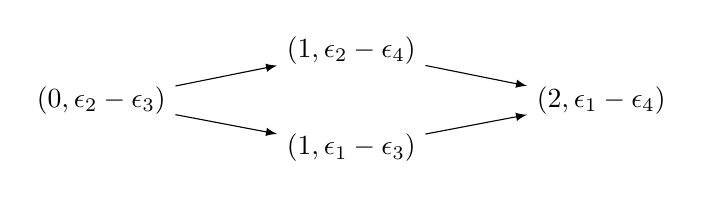
\begin{tikzpicture}[>=latex,line join=bevel,]
%%
\node (node_3) at (117.0bp,43.5bp) [draw,draw=none] {$(1, \epsilon_{2} - \epsilon_{4})$};
  \node (node_2) at (117.0bp,8.5bp) [draw,draw=none] {$(1, \epsilon_{1} - \epsilon_{3})$};
  \node (node_1) at (207.0bp,25.5bp) [draw,draw=none] {$(2, \epsilon_{1} - \epsilon_{4})$};
  \node (node_0) at (27.0bp,25.5bp) [draw,draw=none] {$(0, \epsilon_{2} - \epsilon_{3})$};
  \draw [black,->] (node_2) ..controls (152.39bp,15.144bp) and (161.31bp,16.867bp)  .. (node_1);
  \draw [black,->] (node_0) ..controls (62.481bp,32.553bp) and (71.507bp,34.399bp)  .. (node_3);
  \draw [black,->] (node_0) ..controls (62.393bp,18.856bp) and (71.311bp,17.133bp)  .. (node_2);
  \draw [black,->] (node_3) ..controls (152.48bp,36.447bp) and (161.51bp,34.601bp)  .. (node_1);
%
\end{tikzpicture}
  \caption{Nonnegative scalar products with noncompact roots}
\end{figure}

%\noindent $\lambda = $ $-\omega_{2}$ \\
\noindent Set of singular roots: $\{\epsilon_{2} - \epsilon_{3}$\} \\

\begin{figure}[H]
  \centering
  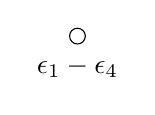
\begin{tikzpicture}
\draw[fill=white] (0 cm, 0 cm) circle (.1cm) node[below=4pt]{$\epsilon_{1} - \epsilon_{4}$};
\end{tikzpicture}
  \caption{The reduced hermitian symmetric pair $(\mathfrak{g}_\lambda, \mathfrak{k}_\lambda)$}
\end{figure}

\begin{figure}[H]
  \centering
      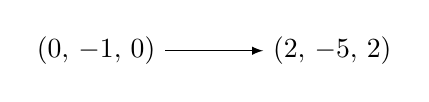
\begin{tikzpicture}[>=latex,line join=bevel,]
%%
\node (node_1) at (24.5bp,8.5bp) [draw,draw=none] {$\left(0,\,-1,\,0\right)$};
  \node (node_0) at (109.5bp,8.5bp) [draw,draw=none] {$\left(2,\,-5,\,2\right)$};
  \draw [black,->] (node_1) ..controls (57.035bp,8.5bp) and (66.102bp,8.5bp)  .. (node_0);
%
\end{tikzpicture}
  \caption{Nilpotent cohomology / BGG resolution}
\end{figure}

        


\subsection[su(1,4): 1,1,1]{$\boldsymbol{\mathfrak{su}(1, 4)\!:\; p'= 1,\, q' = 1,\, l = 1}$}

Cone of unitarizable weights: $-\left(a_{2} + a_{3} + a_{4} + 4\right)\omega_{1} + \left(a_{4} + 1\right)\omega_{4}$ \\


\begin{figure}[H]
  \centering
      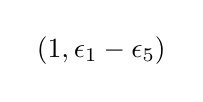
\begin{tikzpicture}[>=latex,line join=bevel,]
%%
\node (node_0) at (27.0bp,8.5bp) [draw,draw=none] {$(1, \epsilon_{1} - \epsilon_{5})$};
%
\end{tikzpicture}
  \caption{Nonnegative scalar products with noncompact roots}
\end{figure}
    

%\noindent $\lambda = $ $-\left(a_{2} + a_{3} + a_{4} + 4\right)\omega_{1} + \left(a_{4} + 1\right)\omega_{4}$ \\
\noindent Set of singular roots: $\emptyset$ \\

\begin{figure}[H]
  \centering
  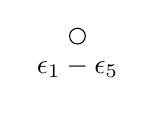
\begin{tikzpicture}
\draw[fill=white] (0 cm, 0 cm) circle (.1cm) node[below=4pt]{$\epsilon_{1} - \epsilon_{5}$};
\end{tikzpicture}
  \caption{The reduced hermitian symmetric pair $(\mathfrak{g}_\lambda, \mathfrak{k}_\lambda)$}
\end{figure}

\begin{figure}[H]
  \centering
      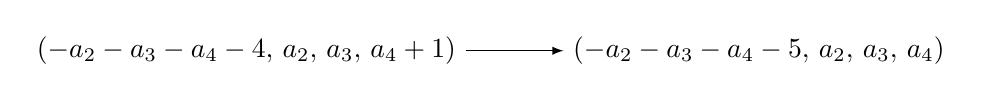
\begin{tikzpicture}[>=latex,line join=bevel,]
%%
\node (node_1) at (263.0bp,8.5bp) [draw,draw=none] {$\left(-a_{2} - a_{3} - a_{4} - 5,\,a_{2},\,a_{3},\,a_{4}\right)$};
  \node (node_0) at (78.5bp,8.5bp) [draw,draw=none] {$\left(-a_{2} - a_{3} - a_{4} - 4,\,a_{2},\,a_{3},\,a_{4} + 1\right)$};
  \draw [black,->] (node_0) ..controls (165.58bp,8.5bp) and (174.15bp,8.5bp)  .. (node_1);
%
\end{tikzpicture}
  \caption{Nilpotent cohomology / BGG resolution}
\end{figure}

        


\subsection[su(1,4): 1,2,1]{$\boldsymbol{\mathfrak{su}(1, 4)\!:\; p'= 1,\, q' = 2,\, l = 1}$}

Cone of unitarizable weights: $-\left(a_{2} + a_{3} + 3\right)\omega_{1} + \left(a_{3} + 1\right)\omega_{3}$ \\


\begin{figure}[H]
  \centering
      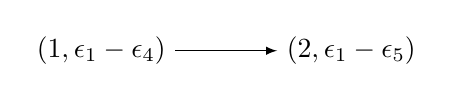
\begin{tikzpicture}[>=latex,line join=bevel,]
%%
\node (node_1) at (117.0bp,8.5bp) [draw,draw=none] {$(2, \epsilon_{1} - \epsilon_{5})$};
  \node (node_0) at (27.0bp,8.5bp) [draw,draw=none] {$(1, \epsilon_{1} - \epsilon_{4})$};
  \draw [black,->] (node_0) ..controls (62.393bp,8.5bp) and (71.311bp,8.5bp)  .. (node_1);
%
\end{tikzpicture}
  \caption{Nonnegative scalar products with noncompact roots}
\end{figure}
    

%\noindent $\lambda = $ $-\left(a_{2} + a_{3} + 3\right)\omega_{1} + \left(a_{3} + 1\right)\omega_{3}$ \\
\noindent Set of singular roots: $\emptyset$ \\

\begin{figure}[H]
  \centering
  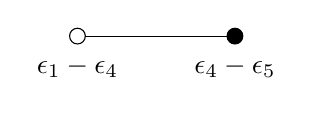
\begin{tikzpicture}
\draw (0 cm,0) -- (2 cm,0);
\draw[fill=white] (0 cm, 0 cm) circle (.1cm) node[below=4pt]{$\epsilon_{1} - \epsilon_{4}$};
\draw[fill=black] (2 cm, 0 cm) circle (.1cm) node[below=4pt]{$\epsilon_{4} - \epsilon_{5}$};
\end{tikzpicture}
  \caption{The reduced hermitian symmetric pair $(\mathfrak{g}_\lambda, \mathfrak{k}_\lambda)$}
\end{figure}

\begin{figure}[H]
  \centering
\begin{tikzpicture}[>=latex,line join=bevel,]
%%
  \node [draw,draw=none] (node_0) at (0, 1) {$\left(-a_{2} - a_{3} - 3,\,a_{2},\,a_{3} + 1,\,0\right)$};
  \node (node_1) at (4, 0) [draw,draw=none] {$\left(-a_{2} - a_{3} - 4,\,a_{2},\,a_{3},\,1\right)$};
  \node [draw,draw=none] (node_2) at (8,-1) {$\left(-a_{2} - a_{3} - 5,\,a_{2},\,a_{3},\,0\right)$};
  \draw  [black,->] (node_0) edge (node_1);
  \draw  [black,->] (node_1) edge (node_2);
\end{tikzpicture}
  \caption{Nilpotent cohomology / BGG resolution}
\end{figure}



\subsection[su(1,4): 1,3,1]{$\boldsymbol{\mathfrak{su}(1, 4)\!:\; p'= 1,\, q' = 3,\, l = 1}$}

Cone of unitarizable weights: $-\left(a_{2} + 2\right)\omega_{1} + \left(a_{2} + 1\right)\omega_{2}$ \\


\begin{figure}[H]
  \centering
      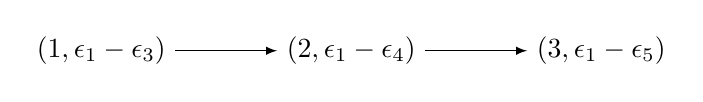
\begin{tikzpicture}[>=latex,line join=bevel,]
%%
\node (node_2) at (117.0bp,8.5bp) [draw,draw=none] {$(2, \epsilon_{1} - \epsilon_{4})$};
  \node (node_1) at (27.0bp,8.5bp) [draw,draw=none] {$(1, \epsilon_{1} - \epsilon_{3})$};
  \node (node_0) at (207.0bp,8.5bp) [draw,draw=none] {$(3, \epsilon_{1} - \epsilon_{5})$};
  \draw [black,->] (node_2) ..controls (152.39bp,8.5bp) and (161.31bp,8.5bp)  .. (node_0);
  \draw [black,->] (node_1) ..controls (62.393bp,8.5bp) and (71.311bp,8.5bp)  .. (node_2);
%
\end{tikzpicture}
  \caption{Nonnegative scalar products with noncompact roots}
\end{figure}
    

%\noindent $\lambda = $ $-\left(a_{2} + 2\right)\omega_{1} + \left(a_{2} + 1\right)\omega_{2}$ \\
\noindent Set of singular roots: $\emptyset$ \\

\begin{figure}[H]
  \centering
  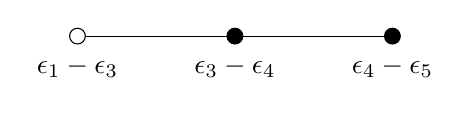
\begin{tikzpicture}
\draw (0 cm,0) -- (4 cm,0);
\draw[fill=white] (0 cm, 0 cm) circle (.1cm) node[below=4pt]{$\epsilon_{1} - \epsilon_{3}$};
\draw[fill=black] (2 cm, 0 cm) circle (.1cm) node[below=4pt]{$\epsilon_{3} - \epsilon_{4}$};
\draw[fill=black] (4 cm, 0 cm) circle (.1cm) node[below=4pt]{$\epsilon_{4} - \epsilon_{5}$};
\end{tikzpicture}
  \caption{The reduced hermitian symmetric pair $(\mathfrak{g}_\lambda, \mathfrak{k}_\lambda)$}
\end{figure}

\begin{figure}[H]
  \centering
      \begin{tikzpicture}[>=latex,line join=bevel,]
%%
  \node (node_2) at (6,0) [draw,draw=none] {$\left(-a_{2} - 4,\,a_{2},\,0,\,1\right)$};
  \node (node_1) at (3,1) [draw,draw=none] {$\left(-a_{2} - 3,\,a_{2},\,1,\,0\right)$};
  \node (node_3) at (9, -1) [draw,draw=none] {$\left(-a_{2} - 5,\,a_{2},\,0,\,0\right)$};
  \node (node_0) at (0, 2) [draw,draw=none] {$\left(-a_{2} - 2,\,a_{2} + 1,\,0,\,0\right)$};

  \draw [black,->] (node_0) edge (node_1);  
  \draw [black,->] (node_1) edge (node_2);  
  \draw [black,->] (node_2) edge (node_3);  
  
\end{tikzpicture}
  \caption{Nilpotent cohomology / BGG resolution}
\end{figure}

        


\subsection[su(1,4): 1,4,1]{$\boldsymbol{\mathfrak{su}(1, 4)\!:\; p'= 1,\, q' = 4,\, l = 1}$}

Cone of unitarizable weights: $0$ \\


\begin{figure}[H]
  \centering
      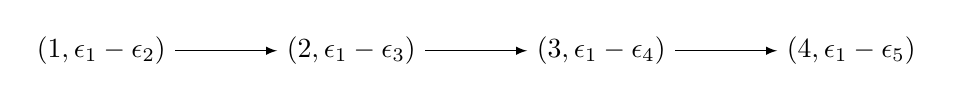
\begin{tikzpicture}[>=latex,line join=bevel,]
%%
\node (node_3) at (207.0bp,8.5bp) [draw,draw=none] {$(3, \epsilon_{1} - \epsilon_{4})$};
  \node (node_2) at (117.0bp,8.5bp) [draw,draw=none] {$(2, \epsilon_{1} - \epsilon_{3})$};
  \node (node_1) at (27.0bp,8.5bp) [draw,draw=none] {$(1, \epsilon_{1} - \epsilon_{2})$};
  \node (node_0) at (297.0bp,8.5bp) [draw,draw=none] {$(4, \epsilon_{1} - \epsilon_{5})$};
  \draw [black,->] (node_3) ..controls (242.39bp,8.5bp) and (251.31bp,8.5bp)  .. (node_0);
  \draw [black,->] (node_2) ..controls (152.39bp,8.5bp) and (161.31bp,8.5bp)  .. (node_3);
  \draw [black,->] (node_1) ..controls (62.393bp,8.5bp) and (71.311bp,8.5bp)  .. (node_2);
%
\end{tikzpicture}
  \caption{Nonnegative scalar products with noncompact roots}
\end{figure}

%\noindent $\lambda = $ $0$ \\
\noindent Set of singular roots: $\emptyset$ \\

\begin{figure}[H]
  \centering
  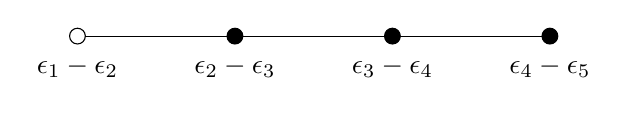
\begin{tikzpicture}
\draw (0 cm,0) -- (6 cm,0);
\draw[fill=white] (0 cm, 0 cm) circle (.1cm) node[below=4pt]{$\epsilon_{1} - \epsilon_{2}$};
\draw[fill=black] (2 cm, 0 cm) circle (.1cm) node[below=4pt]{$\epsilon_{2} - \epsilon_{3}$};
\draw[fill=black] (4 cm, 0 cm) circle (.1cm) node[below=4pt]{$\epsilon_{3} - \epsilon_{4}$};
\draw[fill=black] (6 cm, 0 cm) circle (.1cm) node[below=4pt]{$\epsilon_{4} - \epsilon_{5}$};
\end{tikzpicture}
  \caption{The reduced hermitian symmetric pair $(\mathfrak{g}_\lambda, \mathfrak{k}_\lambda)$}
\end{figure}

\begin{figure}[H]
  \centering
      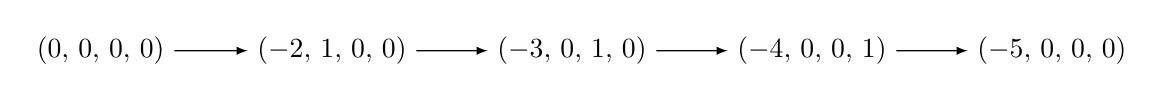
\begin{tikzpicture}[>=latex,line join=bevel,scale=0.9]
%%
\node (node_4) at (215.0bp,8.5bp) [draw,draw=none] {$\left(-3,\,0,\,1,\,0\right)$};
  \node (node_3) at (311.0bp,8.5bp) [draw,draw=none] {$\left(-4,\,0,\,0,\,1\right)$};
  \node (node_2) at (26.5bp,8.5bp) [draw,draw=none] {$\left(0,\,0,\,0,\,0\right)$};
  \node (node_1) at (407.0bp,8.5bp) [draw,draw=none] {$\left(-5,\,0,\,0,\,0\right)$};
  \node (node_0) at (119.0bp,8.5bp) [draw,draw=none] {$\left(-2,\,1,\,0,\,0\right)$};
  \draw [black,->] (node_0) ..controls (157.27bp,8.5bp) and (166.13bp,8.5bp)  .. (node_4);
  \draw [black,->] (node_2) ..controls (61.068bp,8.5bp) and (69.923bp,8.5bp)  .. (node_0);
  \draw [black,->] (node_4) ..controls (253.27bp,8.5bp) and (262.13bp,8.5bp)  .. (node_3);
  \draw [black,->] (node_3) ..controls (349.27bp,8.5bp) and (358.13bp,8.5bp)  .. (node_1);
%
\end{tikzpicture}
  \caption{Nilpotent cohomology / BGG resolution}
\end{figure}

        


\subsection[su(2,3): 1,1,1]{$\boldsymbol{\mathfrak{su}(2, 3)\!:\; p'= 1,\, q' = 1,\, l = 1}$}

Cone of unitarizable weights: $\left(a_{1} + 1\right)\omega_{1} - \left(a_{1} + a_{3} + a_{4} + 5\right)\omega_{2} + \left(a_{4} + 1\right)\omega_{4}$ \\


\begin{figure}[H]
  \centering
      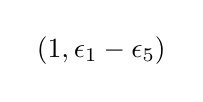
\begin{tikzpicture}[>=latex,line join=bevel,]
%%
\node (node_0) at (27.0bp,8.5bp) [draw,draw=none] {$(1, \epsilon_{1} - \epsilon_{5})$};
%
\end{tikzpicture}
  \caption{Nonnegative scalar products with noncompact roots}
\end{figure}
    

%\noindent $\lambda = $ $\left(a_{1} + 1\right)\omega_{1} - \left(a_{1} + a_{3} + a_{4} + 5\right)\omega_{2} + \left(a_{4} + 1\right)\omega_{4}$ \\
\noindent Set of singular roots: $\emptyset$ \\

\begin{figure}[H]
  \centering
  \begin{tikzpicture}
\draw[fill=white] (0 cm, 0 cm) circle (.1cm) node[below=4pt]{$\epsilon_{1} - \epsilon_{5}$};
\end{tikzpicture}
  \caption{The reduced hermitian symmetric pair $(\mathfrak{g}_\lambda, \mathfrak{k}_\lambda)$}
\end{figure}

\begin{figure}[H]
  \centering
      \begin{tikzpicture}[>=latex,line join=bevel,]
%%
\node (node_1) at (87.5bp,8.5bp) [draw,draw=none] {$\left(a_{1} + 1,\,-a_{1} - a_{3} - a_{4} - 5,\,a_{3},\,a_{4} + 1\right)$};
  \node (node_0) at (281.0bp,8.5bp) [draw,draw=none] {$\left(a_{1},\,-a_{1} - a_{3} - a_{4} - 5,\,a_{3},\,a_{4}\right)$};
  \draw [black,->] (node_1) ..controls (183.53bp,8.5bp) and (192.16bp,8.5bp)  .. (node_0);
%
\end{tikzpicture}
  \caption{Nilpotent cohomology / BGG resolution}
\end{figure}

        


\subsection[su(2,3): 1,2,1]{$\boldsymbol{\mathfrak{su}(2, 3)\!:\; p'= 1,\, q' = 2,\, l = 1}$}

Cone of unitarizable weights: $\left(a_{1} + 1\right)\omega_{1} - \left(a_{1} + a_{3} + 4\right)\omega_{2} + \left(a_{3} + 1\right)\omega_{3}$ \\


\begin{figure}[H]
  \centering
      \begin{tikzpicture}[>=latex,line join=bevel,]
%%
\node (node_2) at (130.0bp,25.5bp) [draw,draw=none] {$(2, \epsilon_{1} - \epsilon_{5})$};
  \node (node_1) at (33.5bp,8.5bp) [draw,draw=none] {$(1, \epsilon_{1} - \epsilon_{4})$};
  \node (node_0) at (33.5bp,43.5bp) [draw,draw=none] {$(-a_{1}, \epsilon_{2} - \epsilon_{5})$};
  \draw [black,->] (node_0) ..controls (75.372bp,35.715bp) and (84.404bp,33.994bp)  .. (node_2);
  \draw [black,->] (node_1) ..controls (70.509bp,14.978bp) and (82.02bp,17.049bp)  .. (node_2);
%
\end{tikzpicture}
  \caption{Nonnegative scalar products with noncompact roots}
\end{figure}
    

\noindent $\lambda = \omega_{1} - \left(a_{3} + 4\right)\omega_{2} + \left(a_{3} + 1\right)\omega_{3}$ \\
\noindent Set of singular roots: $\{\epsilon_{2} - \epsilon_{5}$\} \\

\begin{figure}[H]
  \centering
  \begin{tikzpicture}
\draw[fill=white] (0 cm, 0 cm) circle (.1cm) node[below=4pt]{$\epsilon_{1} - \epsilon_{4}$};
\end{tikzpicture}
  \caption{The reduced hermitian symmetric pair $(\mathfrak{g}_\lambda, \mathfrak{k}_\lambda)$}
\end{figure}

\begin{figure}[H]
  \centering
      \begin{tikzpicture}[>=latex,line join=bevel,]
%%
\node (node_1) at (241.0bp,8.5bp) [draw,draw=none] {$\left(0,\, - a_{3} - 4,\,a_{3},\,1\right)$};
  \node (node_0) at (74.0bp,8.5bp) [draw,draw=none] {$\left(1,\,- a_{3} - 4,\,a_{3} + 1,\,0\right)$};
  \draw [black,->] (node_0) ..controls (156.78bp,8.5bp) and (165.35bp,8.5bp)  .. (node_1);
%
\end{tikzpicture}
  \caption{Nilpotent cohomology / BGG resolution}
\end{figure}

\noindent $\lambda = \left(a_{1} + 1\right)\omega_{1} - \left(a_{1} + a_{3} + 4\right)\omega_{2} + \left(a_{3} + 1\right)\omega_{3}$, $a_{1} \geq 1$ \\
\noindent Set of singular roots: $\emptyset$ \\

\begin{figure}[H]
  \centering
  \begin{tikzpicture}
\draw (0 cm,0) -- (2 cm,0);
\draw[fill=white] (0 cm, 0 cm) circle (.1cm) node[below=4pt]{$\epsilon_{1} - \epsilon_{4}$};
\draw[fill=black] (2 cm, 0 cm) circle (.1cm) node[below=4pt]{$\epsilon_{4} - \epsilon_{5}$};
\end{tikzpicture}
  \caption{The reduced hermitian symmetric pair $(\mathfrak{g}_\lambda, \mathfrak{k}_\lambda)$}
\end{figure}

\begin{figure}[H]
  \centering
      \begin{tikzpicture}[>=latex,line join=bevel,]
%%
\node (node_1) at (4,0) [draw,draw=none] {$\left(a_{1},\,-a_{1} - a_{3} - 4,\,a_{3},\,1\right)$};
  \node (node_0) at (0, 1) [draw,draw=none] {$\left(a_{1} + 1,\,-a_{1} - a_{3} - 4,\,a_{3} + 1,\,0\right)$};
  \node (node_2) at (8, -1) [draw,draw=none] {$\left(a_{1} - 1,\,-a_{1} - a_{3} - 4,\,a_{3},\,0\right)$};
  \draw [black,->] (node_0) edge (node_1);
  \draw [black,->] (node_1) edge (node_2);
%
\end{tikzpicture}
  \caption{Nilpotent cohomology / BGG resolution}
\end{figure}


\subsection[su(2,3): 1,3,1]{$\boldsymbol{\mathfrak{su}(2, 3)\!:\; p'= 1,\, q' = 3,\, l = 1}$}

Cone of unitarizable weights: $\left(a_{1} + 1\right)\omega_{1} - \left(a_{1} + 2\right)\omega_{2}$ \\


\begin{figure}[H]
  \centering
      \begin{tikzpicture}[>=latex,line join=bevel,]
%%
\node (node_4) at (33.5bp,43.5bp) [draw,draw=none] {$(-a_{1}, \epsilon_{2} - \epsilon_{4})$};
  \node (node_3) at (145.0bp,8.5bp) [draw,draw=none] {$(2, \epsilon_{1} - \epsilon_{4})$};
  \node (node_2) at (145.0bp,43.5bp) [draw,draw=none] {$(-a_{1} + 1, \epsilon_{2} - \epsilon_{5})$};
  \node (node_1) at (33.5bp,8.5bp) [draw,draw=none] {$(1, \epsilon_{1} - \epsilon_{3})$};
  \node (node_0) at (250.0bp,25.5bp) [draw,draw=none] {$(3, \epsilon_{1} - \epsilon_{5})$};
  \draw [black,->] (node_1) ..controls (74.814bp,8.5bp) and (92.394bp,8.5bp)  .. (node_3);
  \draw [black,->] (node_3) ..controls (184.61bp,14.872bp) and (199.53bp,17.335bp)  .. (node_0);
  \draw [black,->] (node_2) ..controls (195.62bp,34.829bp) and (204.64bp,33.252bp)  .. (node_0);
  \draw [black,->] (node_4) ..controls (75.414bp,30.423bp) and (92.936bp,24.822bp)  .. (node_3);
  \draw [black,->] (node_4) ..controls (75.123bp,43.5bp) and (83.962bp,43.5bp)  .. (node_2);
%
\end{tikzpicture}
  \caption{Nonnegative scalar products with noncompact roots}
\end{figure}
    
% a1 = 0
\noindent $\lambda = \omega_{1} - 2\omega_{2}$ \\
\noindent Set of singular roots: $\{\epsilon_{2} - \epsilon_{4}$\} \\

\begin{figure}[H]
  \centering
  \begin{tikzpicture}
\draw (0 cm,0) -- (2 cm,0);
\draw[fill=white] (0 cm, 0 cm) circle (.1cm) node[below=4pt]{$\epsilon_{1} - \epsilon_{3}$};
\draw[fill=black] (2 cm, 0 cm) circle (.1cm) node[below=4pt]{$\epsilon_{3} - \epsilon_{5}$};
\end{tikzpicture}
  \caption{The reduced hermitian symmetric pair $(\mathfrak{g}_\lambda, \mathfrak{k}_\lambda)$}
\end{figure}

\begin{figure}[H]
  \centering
      \begin{tikzpicture}[>=latex,line join=bevel,]
%%
\node (node_2) at (52.0bp,8.5bp) [draw,draw=none] {$\left(1,\, - 2,\,0,\,0\right)$};
  \node (node_1) at (183.5bp,8.5bp) [draw,draw=none] {$\left(0,\,- 3,\,1,\,0\right)$};
  \node (node_0) at (315.0bp,8.5bp) [draw,draw=none] {$\left( - 2,\, - 4,\,1,\,1\right)$};
  \draw [black,->] (node_2) ..controls (112.53bp,8.5bp) and (121.18bp,8.5bp)  .. (node_1);
  \draw [black,->] (node_1) ..controls (235.42bp,8.5bp) and (244.1bp,8.5bp)  .. (node_0);
%
\end{tikzpicture}
  \caption{Nilpotent cohomology / BGG resolution}
\end{figure}

% a1 = 1
\noindent $\lambda = 2\omega_{1} - 3\omega_{2}$ \\
\noindent Set of singular roots: $\{\epsilon_{2} - \epsilon_{5}$\} \\

\begin{figure}[H]
  \centering
  \begin{tikzpicture}
\draw (0 cm,0) -- (2 cm,0);
\draw[fill=white] (0 cm, 0 cm) circle (.1cm) node[below=4pt]{$\epsilon_{1} - \epsilon_{3}$};
\draw[fill=black] (2 cm, 0 cm) circle (.1cm) node[below=4pt]{$\epsilon_{3} - \epsilon_{4}$};
\end{tikzpicture}
  \caption{The reduced hermitian symmetric pair $(\mathfrak{g}_\lambda, \mathfrak{k}_\lambda)$}
\end{figure}

\begin{figure}[H]
  \centering
      \begin{tikzpicture}[>=latex,line join=bevel,]
%%
\node (node_2) at (183.5bp,8.5bp) [draw,draw=none] {$\left(1,\,-4,\,1,\,0\right)$};
  \node (node_1) at (315.0bp,8.5bp) [draw,draw=none] {$\left(0,\,-4,\,0,\,1\right)$};
  \node (node_0) at (52.0bp,8.5bp) [draw,draw=none] {$\left(2,\,-3,\,0,\,0\right)$};
  \draw [black,->] (node_2) ..controls (235.42bp,8.5bp) and (244.1bp,8.5bp)  .. (node_1);
  \draw [black,->] (node_0) ..controls (112.53bp,8.5bp) and (121.18bp,8.5bp)  .. (node_2);
%
\end{tikzpicture}
  \caption{Nilpotent cohomology / BGG resolution}
\end{figure}
        
\noindent $\lambda = \left(a_{1} + 1\right)\omega_{1} - \left(a_{1} + 2\right)\omega_{2}$, $a_1 \geq 2$ \\
\noindent Set of singular roots: $\emptyset$ \\

\begin{figure}[H]
  \centering
  \begin{tikzpicture}
\draw (0 cm,0) -- (4 cm,0);
\draw[fill=white] (0 cm, 0 cm) circle (.1cm) node[below=4pt]{$\epsilon_{1} - \epsilon_{3}$};
\draw[fill=black] (2 cm, 0 cm) circle (.1cm) node[below=4pt]{$\epsilon_{3} - \epsilon_{4}$};
\draw[fill=black] (4 cm, 0 cm) circle (.1cm) node[below=4pt]{$\epsilon_{4} - \epsilon_{5}$};
\end{tikzpicture}
  \caption{The reduced hermitian symmetric pair $(\mathfrak{g}_\lambda, \mathfrak{k}_\lambda)$}
\end{figure}

\begin{figure}[H]
  \centering
      \begin{tikzpicture}[>=latex,line join=bevel,]
%%
\node (node_1) at (3,2) [draw,draw=none] {$\left(a_{1},\,-a_{1} - 3,\,1,\,0\right)$};
  \node (node_3) at (9,0) [draw,draw=none] {$\left(a_{1} - 2,\,-a_{1} - 3,\,0,\,0\right)$};
  \node (node_2) at (6,1) [draw,draw=none] {$\left(a_{1} - 1,\,-a_{1} - 3,\,0,\,1\right)$};
  \node (node_0) at (0,3) [draw,draw=none] {$\left(a_{1} + 1,\,-a_{1} - 2,\,0,\,0\right)$};
  \draw [black,->] (node_0) edge (node_1);
  \draw [black,->] (node_1) edge (node_2);
  \draw [black,->] (node_2) edge (node_3);
%
\end{tikzpicture}
  \caption{Nilpotent cohomology / BGG resolution}
\end{figure}

\subsection[su(2,3): 2,1,1]{$\boldsymbol{\mathfrak{su}(2, 3)\!:\; p'= 2,\, q' = 1,\, l = 1}$}

Cone of unitarizable weights: $-\left(a_{3} + a_{4} + 3\right)\omega_{2} + \left(a_{4} + 1\right)\omega_{4}$ \\


\begin{figure}[H]
  \centering
      \begin{tikzpicture}[>=latex,line join=bevel,]
%%
\node (node_2) at (33.5bp,43.5bp) [draw,draw=none] {$(-a_{4}, \epsilon_{1} - \epsilon_{4})$};
  \node (node_1) at (33.5bp,8.5bp) [draw,draw=none] {$(1, \epsilon_{2} - \epsilon_{5})$};
  \node (node_0) at (130.0bp,25.5bp) [draw,draw=none] {$(2, \epsilon_{1} - \epsilon_{5})$};
  \draw [black,->] (node_2) ..controls (75.372bp,35.715bp) and (84.404bp,33.994bp)  .. (node_0);
  \draw [black,->] (node_1) ..controls (70.509bp,14.978bp) and (82.02bp,17.049bp)  .. (node_0);
%
\end{tikzpicture}
  \caption{Nonnegative scalar products with noncompact roots}
\end{figure}
    

\noindent $\lambda = $ $-\left(a_{3} +  3\right)\omega_{2} + \omega_{4}$ \\
\noindent Set of singular roots: $\{\epsilon_{1} - \epsilon_{4}$\} \\

\begin{figure}[H]
  \centering
  \begin{tikzpicture}
\draw[fill=white] (0 cm, 0 cm) circle (.1cm) node[below=4pt]{$\epsilon_{2} - \epsilon_{5}$};
\end{tikzpicture}
  \caption{The reduced hermitian symmetric pair $(\mathfrak{g}_\lambda, \mathfrak{k}_\lambda)$}
\end{figure}

\begin{figure}[H]
  \centering
      \begin{tikzpicture}[>=latex,line join=bevel,]
%%
\node (node_1) at (224.0bp,8.5bp) [draw,draw=none] {$\left(1,\,-a_{3} - 4,\,a_{3},\,0\right)$};
  \node (node_0) at (65.5bp,8.5bp) [draw,draw=none] {$\left(0,\,-a_{3}  - 3,\,a_{3},\, 1\right)$};
  \draw [black,->] (node_0) ..controls (139.44bp,8.5bp) and (148.04bp,8.5bp)  .. (node_1);
%
\end{tikzpicture}
  \caption{Nilpotent cohomology / BGG resolution}
\end{figure}

\noindent $\lambda = $ $-\left(a_{3} + a_{4} + 3\right)\omega_{2} + \left(a_{4} + 1\right)\omega_{4}$, $a_4 \geq 1$ \\
\noindent Set of singular roots: $\emptyset$ \\

\begin{figure}[H]
  \centering
  \begin{tikzpicture}
\draw (0 cm,0) -- (2 cm,0);
\draw[fill=black] (0 cm, 0 cm) circle (.1cm) node[below=4pt]{$\epsilon_{1} - \epsilon_{2}$};
\draw[fill=white] (2 cm, 0 cm) circle (.1cm) node[below=4pt]{$\epsilon_{2} - \epsilon_{5}$};
\end{tikzpicture}
  \caption{The reduced hermitian symmetric pair $(\mathfrak{g}_\lambda, \mathfrak{k}_\lambda)$}
\end{figure}

\begin{figure}[H]
  \centering
      \begin{tikzpicture}[>=latex,line join=bevel,]
%%
\node (node_1) at (4,1) [draw,draw=none] {$\left(1,\,-a_{3} - a_{4} - 4,\,a_{3},\,a_{4}\right)$};
  \node (node_0) at (0,2) [draw,draw=none] {$\left(0,\,-a_{3} - a_{4} - 3,\,a_{3},\,a_{4} + 1\right)$};
  \node (node_2) at (8,0) [draw,draw=none] {$\left(0,\,-a_{3} - a_{4} - 4,\,a_{3},\,a_{4} - 1\right)$};
  \draw [black,->] (node_0) edge (node_1);
  \draw [black,->] (node_1) edge (node_2);
%
\end{tikzpicture}
  \caption{Nilpotent cohomology / BGG resolution}
\end{figure}        


\subsection[su(2,3): 2,2,1]{$\boldsymbol{\mathfrak{su}(2, 3)\!:\; p'= 2,\, q' = 2,\, l = 1}$}

Cone of unitarizable weights: $-\left(a_{3} + 2\right)\omega_{2} + \left(a_{3} + 1\right)\omega_{3}$ \\


\begin{figure}[H]
  \centering
      \begin{tikzpicture}[>=latex,line join=bevel,]
%%
\node (node_4) at (33.5bp,8.5bp) [draw,draw=none] {$(1, \epsilon_{2} - \epsilon_{4})$};
  \node (node_3) at (220.0bp,25.5bp) [draw,draw=none] {$(3, \epsilon_{1} - \epsilon_{5})$};
  \node (node_2) at (130.0bp,8.5bp) [draw,draw=none] {$(2, \epsilon_{2} - \epsilon_{5})$};
  \node (node_1) at (33.5bp,43.5bp) [draw,draw=none] {$(-a_{3}, \epsilon_{1} - \epsilon_{3})$};
  \node (node_0) at (130.0bp,43.5bp) [draw,draw=none] {$(2, \epsilon_{1} - \epsilon_{4})$};
  \draw [black,->] (node_0) ..controls (165.48bp,36.447bp) and (174.51bp,34.601bp)  .. (node_3);
  \draw [black,->] (node_4) ..controls (69.418bp,21.432bp) and (83.564bp,26.672bp)  .. (node_0);
  \draw [black,->] (node_2) ..controls (165.39bp,15.144bp) and (174.31bp,16.867bp)  .. (node_3);
  \draw [black,->] (node_1) ..controls (75.372bp,43.5bp) and (84.404bp,43.5bp)  .. (node_0);
  \draw [black,->] (node_4) ..controls (70.406bp,8.5bp) and (81.783bp,8.5bp)  .. (node_2);
%
\end{tikzpicture}
  \caption{Nonnegative scalar products with noncompact roots}
\end{figure}
    

\noindent $\lambda = $ $-2\omega_{2} + \omega_{3}$ \\
\noindent Set of singular roots: $\{\epsilon_{1} - \epsilon_{3}$\} \\

\begin{figure}[H]
  \centering
  \begin{tikzpicture}
\draw (0 cm,0) -- (2 cm,0);
\draw[fill=white] (0 cm, 0 cm) circle (.1cm) node[below=4pt]{$\epsilon_{2} - \epsilon_{4}$};
\draw[fill=black] (2 cm, 0 cm) circle (.1cm) node[below=4pt]{$\epsilon_{4} - \epsilon_{5}$};
\end{tikzpicture}
  \caption{The reduced hermitian symmetric pair $(\mathfrak{g}_\lambda, \mathfrak{k}_\lambda)$}
\end{figure}

\begin{figure}[H]
  \centering
      \begin{tikzpicture}[>=latex,line join=bevel,]
%%
\node (node_2) at (52.0bp,8.5bp) [draw,draw=none] {$\left(0,\, - 2,\,1,\,0\right)$};
  \node (node_1) at (306.5bp,8.5bp) [draw,draw=none] {$\left(2,\, - 4,\,0,\,0\right)$};
  \node (node_0) at (183.5bp,8.5bp) [draw,draw=none] {$\left(1,\, - 3,\,0,\,1\right)$};
  \draw [black,->] (node_0) ..controls (235.38bp,8.5bp) and (244.09bp,8.5bp)  .. (node_1);
  \draw [black,->] (node_2) ..controls (112.53bp,8.5bp) and (121.18bp,8.5bp)  .. (node_0);
%
\end{tikzpicture}
  \caption{Nilpotent cohomology / BGG resolution}
\end{figure}

\noindent $\lambda = $ $-\left(a_{3} + 2\right)\omega_{2} + \left(a_{3} + 1\right)\omega_{3}$, $a_3 \geq 1$ \\
\noindent Set of singular roots: $\emptyset$ \\

\begin{figure}[H]
  \centering
  \begin{tikzpicture}
\draw (0 cm,0) -- (4 cm,0);
\draw[fill=black] (0 cm, 0 cm) circle (.1cm) node[below=4pt]{$\epsilon_{1} - \epsilon_{2}$};
\draw[fill=white] (2 cm, 0 cm) circle (.1cm) node[below=4pt]{$\epsilon_{2} - \epsilon_{4}$};
\draw[fill=black] (4 cm, 0 cm) circle (.1cm) node[below=4pt]{$\epsilon_{4} - \epsilon_{5}$};
\end{tikzpicture}
  \caption{The reduced hermitian symmetric pair $(\mathfrak{g}_\lambda, \mathfrak{k}_\lambda)$}
\end{figure}

\begin{figure}[H]
  \centering
      \begin{tikzpicture}[>=latex,line join=bevel,]
%%
\node (node_5) at (73.0bp,142.0bp) [draw,draw=none] {$ \begin{tikzpicture}\draw (0 cm,0) -- (4.5 cm,0);\draw[fill=black] (0.00 cm, 0 cm) circle (.1cm) node[below=4pt]{$2$};\draw[fill=white] (1.5 cm, 0 cm) circle (.1cm) node[below=4pt]{$-a_{3} - 4$};\draw[fill=black] (3.0 cm, 0 cm) circle (.1cm) node[below=4pt]{$a_{3}$};\draw[fill=black] (4.5 cm, 0 cm) circle (.1cm) node[below=4pt]{$0$};\end{tikzpicture} $};
  \node (node_4) at (155.0bp,270.0bp) [draw,draw=none] {$ \begin{tikzpicture}\draw (0 cm,0) -- (4.5 cm,0);\draw[fill=black] (0.00 cm, 0 cm) circle (.1cm) node[below=4pt]{$0$};\draw[fill=white] (1.5 cm, 0 cm) circle (.1cm) node[below=4pt]{$-a_{3} - 2$};\draw[fill=black] (3.0 cm, 0 cm) circle (.1cm) node[below=4pt]{$a_{3} + 1$};\draw[fill=black] (4.5 cm, 0 cm) circle (.1cm) node[below=4pt]{$0$};\end{tikzpicture} $};
  \node (node_3) at (155.0bp,206.0bp) [draw,draw=none] {$ \begin{tikzpicture}\draw (0 cm,0) -- (4.5 cm,0);\draw[fill=black] (0.00 cm, 0 cm) circle (.1cm) node[below=4pt]{$1$};\draw[fill=white] (1.5 cm, 0 cm) circle (.1cm) node[below=4pt]{$-a_{3} - 3$};\draw[fill=black] (3.0 cm, 0 cm) circle (.1cm) node[below=4pt]{$a_{3}$};\draw[fill=black] (4.5 cm, 0 cm) circle (.1cm) node[below=4pt]{$1$};\end{tikzpicture} $};
  \node (node_2) at (237.0bp,142.0bp) [draw,draw=none] {$ \begin{tikzpicture}\draw (0 cm,0) -- (4.5 cm,0);\draw[fill=black] (0.00 cm, 0 cm) circle (.1cm) node[below=4pt]{$0$};\draw[fill=white] (1.5 cm, 0 cm) circle (.1cm) node[below=4pt]{$-a_{3} - 3$};\draw[fill=black] (3.0 cm, 0 cm) circle (.1cm) node[below=4pt]{$a_{3} - 1$};\draw[fill=black] (4.5 cm, 0 cm) circle (.1cm) node[below=4pt]{$2$};\end{tikzpicture} $};
  \node (node_1) at (155.0bp,14.0bp) [draw,draw=none] {$ \begin{tikzpicture}\draw (0 cm,0) -- (4.5 cm,0);\draw[fill=black] (0.00 cm, 0 cm) circle (.1cm) node[below=4pt]{$0$};\draw[fill=white] (1.5 cm, 0 cm) circle (.1cm) node[below=4pt]{$-a_{3} - 4$};\draw[fill=black] (3.0 cm, 0 cm) circle (.1cm) node[below=4pt]{$a_{3} - 1$};\draw[fill=black] (4.5 cm, 0 cm) circle (.1cm) node[below=4pt]{$0$};\end{tikzpicture} $};
  \node (node_0) at (155.0bp,78.0bp) [draw,draw=none] {$ \begin{tikzpicture}\draw (0 cm,0) -- (4.5 cm,0);\draw[fill=black] (0.00 cm, 0 cm) circle (.1cm) node[below=4pt]{$1$};\draw[fill=white] (1.5 cm, 0 cm) circle (.1cm) node[below=4pt]{$-a_{3} - 4$};\draw[fill=black] (3.0 cm, 0 cm) circle (.1cm) node[below=4pt]{$a_{3} - 1$};\draw[fill=black] (4.5 cm, 0 cm) circle (.1cm) node[below=4pt]{$1$};\end{tikzpicture} $};
  \draw [black,->] (node_3) ..controls (183.7bp,183.3bp) and (198.64bp,172.01bp)  .. (node_2);
  \draw [black,->] (node_2) ..controls (208.3bp,119.3bp) and (193.36bp,108.01bp)  .. (node_0);
  \draw [black,->] (node_5) ..controls (101.7bp,119.3bp) and (116.64bp,108.01bp)  .. (node_0);
  \draw [black,->] (node_3) ..controls (126.3bp,183.3bp) and (111.36bp,172.01bp)  .. (node_5);
  \draw [black,->] (node_0) ..controls (155.0bp,56.453bp) and (155.0bp,46.998bp)  .. (node_1);
  \draw [black,->] (node_4) ..controls (155.0bp,248.45bp) and (155.0bp,239.0bp)  .. (node_3);
%
\end{tikzpicture}
  \caption{Nilpotent cohomology / BGG resolution}
\end{figure}      


\subsection[su(2,3): 2,2,2]{$\boldsymbol{\mathfrak{su}(2, 3)\!:\; p'= 2,\, q' = 2,\, l = 2}$}

Cone of unitarizable weights: $-\left(a_{3} + 3\right)\omega_{2} + \left(a_{3} + 1\right)\omega_{3}$ \\


\begin{figure}[H]
  \centering
      \begin{tikzpicture}[>=latex,line join=bevel,]
%%
\node (node_3) at (207.0bp,25.5bp) [draw,draw=none] {$(2, \epsilon_{1} - \epsilon_{5})$};
  \node (node_2) at (117.0bp,43.5bp) [draw,draw=none] {$(1, \epsilon_{1} - \epsilon_{4})$};
  \node (node_1) at (117.0bp,8.5bp) [draw,draw=none] {$(1, \epsilon_{2} - \epsilon_{5})$};
  \node (node_0) at (27.0bp,25.5bp) [draw,draw=none] {$(0, \epsilon_{2} - \epsilon_{4})$};
  \draw [black,->] (node_1) ..controls (152.39bp,15.144bp) and (161.31bp,16.867bp)  .. (node_3);
  \draw [black,->] (node_2) ..controls (152.48bp,36.447bp) and (161.51bp,34.601bp)  .. (node_3);
  \draw [black,->] (node_0) ..controls (62.481bp,32.553bp) and (71.507bp,34.399bp)  .. (node_2);
  \draw [black,->] (node_0) ..controls (62.393bp,18.856bp) and (71.311bp,17.133bp)  .. (node_1);
%
\end{tikzpicture}
  \caption{Nonnegative scalar products with noncompact roots}
\end{figure}
    

%\noindent $\lambda = $ $-\left(a_{3} + 3\right)\omega_{2} + \left(a_{3} + 1\right)\omega_{3}$ \\
\noindent Set of singular roots: $\{\epsilon_{2} - \epsilon_{4}$\} \\

\begin{figure}[H]
  \centering
  \begin{tikzpicture}
\draw[fill=white] (0 cm, 0 cm) circle (.1cm) node[below=4pt]{$\epsilon_{1} - \epsilon_{5}$};
\end{tikzpicture}
  \caption{The reduced hermitian symmetric pair $(\mathfrak{g}_\lambda, \mathfrak{k}_\lambda)$}
\end{figure}

\begin{figure}[H]
  \centering
      \begin{tikzpicture}[>=latex,line join=bevel,]
%%
\node (node_1) at (52.0bp,8.5bp) [draw,draw=none] {$\left(0,\,-a_{3} - 3,\,a_{3} + 1,\,0\right)$};
  \node (node_0) at (192.0bp,8.5bp) [draw,draw=none] {$\left(2,\,-a_{3} - 5,\,a_{3} - 1,\,2\right)$};
  \draw [black,->] (node_1) ..controls (112.56bp,8.5bp) and (121.08bp,8.5bp)  .. (node_0);
%
\end{tikzpicture}
  \caption{Nilpotent cohomology / BGG resolution}
\end{figure}

        


\subsection[su(2,3): 2,3,1]{$\boldsymbol{\mathfrak{su}(2, 3)\!:\; p'= 2,\, q' = 3,\, l = 1}$}

Cone of unitarizable weights: $0$ \\


\begin{figure}[H]
  \centering
      \begin{tikzpicture}[>=latex,line join=bevel,]
%%
\node (node_5) at (27.0bp,25.5bp) [draw,draw=none] {$(1, \epsilon_{2} - \epsilon_{3})$};
  \node (node_4) at (117.0bp,43.5bp) [draw,draw=none] {$(2, \epsilon_{1} - \epsilon_{3})$};
  \node (node_3) at (117.0bp,8.5bp) [draw,draw=none] {$(2, \epsilon_{2} - \epsilon_{4})$};
  \node (node_2) at (207.0bp,8.5bp) [draw,draw=none] {$(3, \epsilon_{2} - \epsilon_{5})$};
  \node (node_1) at (207.0bp,43.5bp) [draw,draw=none] {$(3, \epsilon_{1} - \epsilon_{4})$};
  \node (node_0) at (297.0bp,25.5bp) [draw,draw=none] {$(4, \epsilon_{1} - \epsilon_{5})$};
  \draw [black,->] (node_5) ..controls (62.481bp,32.553bp) and (71.507bp,34.399bp)  .. (node_4);
  \draw [black,->] (node_3) ..controls (150.41bp,21.39bp) and (163.43bp,26.568bp)  .. (node_1);
  \draw [black,->] (node_3) ..controls (152.39bp,8.5bp) and (161.31bp,8.5bp)  .. (node_2);
  \draw [black,->] (node_2) ..controls (242.39bp,15.144bp) and (251.31bp,16.867bp)  .. (node_0);
  \draw [black,->] (node_5) ..controls (62.393bp,18.856bp) and (71.311bp,17.133bp)  .. (node_3);
  \draw [black,->] (node_1) ..controls (242.48bp,36.447bp) and (251.51bp,34.601bp)  .. (node_0);
  \draw [black,->] (node_4) ..controls (152.39bp,43.5bp) and (161.31bp,43.5bp)  .. (node_1);
%
\end{tikzpicture}
  \caption{Nonnegative scalar products with noncompact roots}
\end{figure}

%\noindent $\lambda = $ $0$ \\
\noindent Set of singular roots: $\emptyset$ \\

\begin{figure}[H]
  \centering
  \begin{tikzpicture}
\draw (0 cm,0) -- (6 cm,0);
\draw[fill=black] (0 cm, 0 cm) circle (.1cm) node[below=4pt]{$\epsilon_{1} - \epsilon_{2}$};
\draw[fill=white] (2 cm, 0 cm) circle (.1cm) node[below=4pt]{$\epsilon_{2} - \epsilon_{3}$};
\draw[fill=black] (4 cm, 0 cm) circle (.1cm) node[below=4pt]{$\epsilon_{3} - \epsilon_{4}$};
\draw[fill=black] (6 cm, 0 cm) circle (.1cm) node[below=4pt]{$\epsilon_{4} - \epsilon_{5}$};
\end{tikzpicture}
  \caption{The reduced hermitian symmetric pair $(\mathfrak{g}_\lambda, \mathfrak{k}_\lambda)$}
\end{figure}

\begin{figure}[H]
  \centering
      \begin{tikzpicture}[>=latex,line join=bevel,]
%%
\node (node_9) at (73.0bp,206.0bp) [draw,draw=none] {$ \begin{tikzpicture}\draw (0 cm,0) -- (4.5 cm,0);\draw[fill=black] (0.00 cm, 0 cm) circle (.1cm) node[below=4pt]{$3$};\draw[fill=white] (1.5 cm, 0 cm) circle (.1cm) node[below=4pt]{$-4$};\draw[fill=black] (3.0 cm, 0 cm) circle (.1cm) node[below=4pt]{$0$};\draw[fill=black] (4.5 cm, 0 cm) circle (.1cm) node[below=4pt]{$0$};\end{tikzpicture} $};
  \node (node_8) at (155.0bp,14.0bp) [draw,draw=none] {$ \begin{tikzpicture}\draw (0 cm,0) -- (4.5 cm,0);\draw[fill=black] (0.00 cm, 0 cm) circle (.1cm) node[below=4pt]{$0$};\draw[fill=white] (1.5 cm, 0 cm) circle (.1cm) node[below=4pt]{$-5$};\draw[fill=black] (3.0 cm, 0 cm) circle (.1cm) node[below=4pt]{$0$};\draw[fill=black] (4.5 cm, 0 cm) circle (.1cm) node[below=4pt]{$0$};\end{tikzpicture} $};
  \node (node_7) at (237.0bp,142.0bp) [draw,draw=none] {$ \begin{tikzpicture}\draw (0 cm,0) -- (4.5 cm,0);\draw[fill=black] (0.00 cm, 0 cm) circle (.1cm) node[below=4pt]{$0$};\draw[fill=white] (1.5 cm, 0 cm) circle (.1cm) node[below=4pt]{$-4$};\draw[fill=black] (3.0 cm, 0 cm) circle (.1cm) node[below=4pt]{$0$};\draw[fill=black] (4.5 cm, 0 cm) circle (.1cm) node[below=4pt]{$2$};\end{tikzpicture} $};
  \node (node_6) at (155.0bp,78.0bp) [draw,draw=none] {$ \begin{tikzpicture}\draw (0 cm,0) -- (4.5 cm,0);\draw[fill=black] (0.00 cm, 0 cm) circle (.1cm) node[below=4pt]{$1$};\draw[fill=white] (1.5 cm, 0 cm) circle (.1cm) node[below=4pt]{$-5$};\draw[fill=black] (3.0 cm, 0 cm) circle (.1cm) node[below=4pt]{$0$};\draw[fill=black] (4.5 cm, 0 cm) circle (.1cm) node[below=4pt]{$1$};\end{tikzpicture} $};
  \node (node_5) at (237.0bp,270.0bp) [draw,draw=none] {$ \begin{tikzpicture}\draw (0 cm,0) -- (4.5 cm,0);\draw[fill=black] (0.00 cm, 0 cm) circle (.1cm) node[below=4pt]{$0$};\draw[fill=white] (1.5 cm, 0 cm) circle (.1cm) node[below=4pt]{$-3$};\draw[fill=black] (3.0 cm, 0 cm) circle (.1cm) node[below=4pt]{$2$};\draw[fill=black] (4.5 cm, 0 cm) circle (.1cm) node[below=4pt]{$0$};\end{tikzpicture} $};
  \node (node_4) at (237.0bp,206.0bp) [draw,draw=none] {$ \begin{tikzpicture}\draw (0 cm,0) -- (4.5 cm,0);\draw[fill=black] (0.00 cm, 0 cm) circle (.1cm) node[below=4pt]{$1$};\draw[fill=white] (1.5 cm, 0 cm) circle (.1cm) node[below=4pt]{$-4$};\draw[fill=black] (3.0 cm, 0 cm) circle (.1cm) node[below=4pt]{$1$};\draw[fill=black] (4.5 cm, 0 cm) circle (.1cm) node[below=4pt]{$1$};\end{tikzpicture} $};
  \node (node_3) at (73.0bp,142.0bp) [draw,draw=none] {$ \begin{tikzpicture}\draw (0 cm,0) -- (4.5 cm,0);\draw[fill=black] (0.00 cm, 0 cm) circle (.1cm) node[below=4pt]{$2$};\draw[fill=white] (1.5 cm, 0 cm) circle (.1cm) node[below=4pt]{$-5$};\draw[fill=black] (3.0 cm, 0 cm) circle (.1cm) node[below=4pt]{$1$};\draw[fill=black] (4.5 cm, 0 cm) circle (.1cm) node[below=4pt]{$0$};\end{tikzpicture} $};
  \node (node_2) at (73.0bp,270.0bp) [draw,draw=none] {$ \begin{tikzpicture}\draw (0 cm,0) -- (4.5 cm,0);\draw[fill=black] (0.00 cm, 0 cm) circle (.1cm) node[below=4pt]{$2$};\draw[fill=white] (1.5 cm, 0 cm) circle (.1cm) node[below=4pt]{$-3$};\draw[fill=black] (3.0 cm, 0 cm) circle (.1cm) node[below=4pt]{$0$};\draw[fill=black] (4.5 cm, 0 cm) circle (.1cm) node[below=4pt]{$1$};\end{tikzpicture} $};
  \node (node_1) at (155.0bp,334.0bp) [draw,draw=none] {$ \begin{tikzpicture}\draw (0 cm,0) -- (4.5 cm,0);\draw[fill=black] (0.00 cm, 0 cm) circle (.1cm) node[below=4pt]{$1$};\draw[fill=white] (1.5 cm, 0 cm) circle (.1cm) node[below=4pt]{$-2$};\draw[fill=black] (3.0 cm, 0 cm) circle (.1cm) node[below=4pt]{$1$};\draw[fill=black] (4.5 cm, 0 cm) circle (.1cm) node[below=4pt]{$0$};\end{tikzpicture} $};
  \node (node_0) at (155.0bp,397.5bp) [draw,draw=none] {$ \begin{tikzpicture}\draw (0 cm,0) -- (4.5 cm,0);\draw[fill=black] (0.00 cm, 0 cm) circle (.1cm) node[below=4pt]{$0$};\draw[fill=white] (1.5 cm, 0 cm) circle (.1cm) node[below=4pt]{$0$};\draw[fill=black] (3.0 cm, 0 cm) circle (.1cm) node[below=4pt]{$0$};\draw[fill=black] (4.5 cm, 0 cm) circle (.1cm) node[below=4pt]{$0$};\end{tikzpicture} $};
  \draw [black,->] (node_7) ..controls (208.3bp,119.3bp) and (193.36bp,108.01bp)  .. (node_6);
  \draw [black,->] (node_1) ..controls (183.7bp,311.3bp) and (198.64bp,300.01bp)  .. (node_5);
  \draw [black,->] (node_5) ..controls (237.0bp,248.45bp) and (237.0bp,239.0bp)  .. (node_4);
  \draw [black,->] (node_4) ..controls (237.0bp,184.45bp) and (237.0bp,175.0bp)  .. (node_7);
  \draw [black,->] (node_3) ..controls (101.7bp,119.3bp) and (116.64bp,108.01bp)  .. (node_6);
  \draw [black,->] (node_1) ..controls (126.3bp,311.3bp) and (111.36bp,300.01bp)  .. (node_2);
  \draw [black,->] (node_2) ..controls (73.0bp,248.45bp) and (73.0bp,239.0bp)  .. (node_9);
  \draw [black,->] (node_9) ..controls (73.0bp,184.45bp) and (73.0bp,175.0bp)  .. (node_3);
  \draw [black,->] (node_0) ..controls (155.0bp,376.43bp) and (155.0bp,367.01bp)  .. (node_1);
  \draw [black,->] (node_2) ..controls (132.65bp,246.45bp) and (166.31bp,233.72bp)  .. (node_4);
  \draw [black,->] (node_4) ..controls (177.35bp,182.45bp) and (143.69bp,169.72bp)  .. (node_3);
  \draw [black,->] (node_6) ..controls (155.0bp,56.453bp) and (155.0bp,46.998bp)  .. (node_8);
%
\end{tikzpicture}
  \caption{Nilpotent cohomology / BGG resolution}
\end{figure}
%        


\subsection[su(2,3): 2,3,2]{$\boldsymbol{\mathfrak{su}(2, 3)\!:\; p'= 2,\, q' = 3,\, l = 2}$}

Cone of unitarizable weights: $-\omega_{2}$ \\

\begin{figure}[H]
  \centering
      \begin{tikzpicture}[>=latex,line join=bevel,]
%%
\node (node_5) at (297.0bp,25.5bp) [draw,draw=none] {$(3, \epsilon_{1} - \epsilon_{5})$};
  \node (node_4) at (207.0bp,8.5bp) [draw,draw=none] {$(2, \epsilon_{2} - \epsilon_{5})$};
  \node (node_3) at (27.0bp,25.5bp) [draw,draw=none] {$(0, \epsilon_{2} - \epsilon_{3})$};
  \node (node_2) at (117.0bp,8.5bp) [draw,draw=none] {$(1, \epsilon_{2} - \epsilon_{4})$};
  \node (node_1) at (207.0bp,43.5bp) [draw,draw=none] {$(2, \epsilon_{1} - \epsilon_{4})$};
  \node (node_0) at (117.0bp,43.5bp) [draw,draw=none] {$(1, \epsilon_{1} - \epsilon_{3})$};
  \draw [black,->] (node_3) ..controls (62.481bp,32.553bp) and (71.507bp,34.399bp)  .. (node_0);
  \draw [black,->] (node_1) ..controls (242.48bp,36.447bp) and (251.51bp,34.601bp)  .. (node_5);
  \draw [black,->] (node_2) ..controls (150.41bp,21.39bp) and (163.43bp,26.568bp)  .. (node_1);
  \draw [black,->] (node_4) ..controls (242.39bp,15.144bp) and (251.31bp,16.867bp)  .. (node_5);
  \draw [black,->] (node_3) ..controls (62.393bp,18.856bp) and (71.311bp,17.133bp)  .. (node_2);
  \draw [black,->] (node_0) ..controls (152.39bp,43.5bp) and (161.31bp,43.5bp)  .. (node_1);
  \draw [black,->] (node_2) ..controls (152.39bp,8.5bp) and (161.31bp,8.5bp)  .. (node_4);
%
\end{tikzpicture}
  \caption{Nonnegative scalar products with noncompact roots}
\end{figure}

%\noindent $\lambda = $ $-\omega_{2}$ \\
\noindent Set of singular roots: $\{\epsilon_{2} - \epsilon_{3}$\} \\

\begin{figure}[H]
  \centering
  \begin{tikzpicture}
\draw (0 cm,0) -- (2 cm,0);
\draw[fill=white] (0 cm, 0 cm) circle (.1cm) node[below=4pt]{$\epsilon_{1} - \epsilon_{4}$};
\draw[fill=black] (2 cm, 0 cm) circle (.1cm) node[below=4pt]{$\epsilon_{4} - \epsilon_{5}$};
\end{tikzpicture}
  \caption{The reduced hermitian symmetric pair $(\mathfrak{g}_\lambda, \mathfrak{k}_\lambda)$}
\end{figure}

\begin{figure}[H]
  \centering
      \begin{tikzpicture}[>=latex,line join=bevel,]
%%
\node (node_2) at (126.0bp,8.5bp) [draw,draw=none] {$\left(2,\,-5,\,2,\,0\right)$};
  \node (node_1) at (30.0bp,8.5bp) [draw,draw=none] {$\left(0,\,-1,\,0,\,0\right)$};
  \node (node_0) at (222.0bp,8.5bp) [draw,draw=none] {$\left(3,\,-6,\,1,\,1\right)$};
  \draw [black,->] (node_2) ..controls (164.27bp,8.5bp) and (173.13bp,8.5bp)  .. (node_0);
  \draw [black,->] (node_1) ..controls (68.273bp,8.5bp) and (77.134bp,8.5bp)  .. (node_2);
%
\end{tikzpicture}
  \caption{Nilpotent cohomology / BGG resolution}
\end{figure}
